\documentclass[answers]{exam}
\usepackage{../MT2024}
\usepackage{graphicx}
\graphicspath{ {./images/} }

\title{Complex Analysis -- Sheet 2\\Branch cuts, Winding number, Cauchy's integral formula}
\author{YOUR NAME HERE :)}
\date{Michaelmas Term 2024}
% accurate as of 02/10/2024


\begin{document}
\maketitle
\begin{questions}

\question%1
Let $\gamma:[0,1] \to \mathbb{C}$ be a $C^{1}$ curve with $\gamma(0)=i$, $\gamma(1)=-i$ such that $\gamma$ does not intersect $(-\infty, 0]$. Calculate the integral \[
	\int_{\gamma} \operatorname{Log}^{2}(z) \mathrm{~d} z.
\]



\question%2
Calculate the integral \[
	\int_{0}^{2 \pi} e^{e^{i t}} \mathrm{~d} t.
\] [\emph{Hint: See it as an integral along a path.}]



\question%3
Green's Theorem states, for a region $D$ in the plane, bounded by (an) oriented closed curve(s) $C$ in $\mathbb{R}^{2}$ and for real-valued $L$ and $M$ with continuous partial derivatives on $D$, then \[
	\int_{C}(L \mathrm{~d} x+M \mathrm{~d} y)=\iint_{D}\left(M_{x}-L_{y}\right) \mathrm{~d} x \mathrm{~d} y.
\]
\begin{parts}
\part%3a
If we assume, for a holomorphic function $f=u+i v$, that $u_{x}, u_{y}, v_{x}, v_{y}$ are continuous, show that Cauchy's Theorem follows from Green's Theorem, that is, show that for a function $f$ which is holomorphic on the interior $D$ of a closed curve $C$, we have $\int_{C} f(z) \mathrm{~d} z=0$.
\part%3b
Bonus question: Why don't we use this proof in the lectures?
\end{parts}



\fullwidth{In the following questions, for $a \in \mathbb{C}, r>0$ we let $\gamma(a, r)$ denote the positively oriented circle centred at $a$ of radius $r$.}



\question%4
Let \[
	f(z)=\frac{5 z^{2}-8}{z^{3}-2 z^{2}}.
\]
\begin{parts}
\part%4a
Determine $\int_{\gamma(0,1)} f(z) \mathrm{~d} z$. [\emph{Hint: Partial fractions decomposition.}]

\part%4b
Describe different closed paths $\gamma$ in $\mathbb{C}$ such that $\int_{\gamma} f(z) \mathrm{~d} z$ equals \[
	\text{(i) }14\pi i,\qquad
	\text{(ii) }-2\pi i.
\]
\end{parts}



\question%5
Let \[
	I=\int_{\gamma(0,1)} \frac{\operatorname{Re} z}{2 z-i} \mathrm{~d} z \qquad \text{and} \qquad J=\int_{0}^{2 \pi} \frac{\cos ^{2} \theta}{5-4 \sin \theta} \mathrm{d} \theta.
\]
\begin{parts}
\part%5a
Using only Cauchy's Integral Formula, evaluate $I$. (\emph{Note that $\operatorname{Re} z$ is not holomorphic.})

\part%5b
By setting $z=e^{i \theta}$ in the integral for $I$, determine $J$.
\end{parts}



\question%6
By making the substitution $z=r e^{i \theta}$, and making clear any special cases, for each integer $k$ determine $\int_{\gamma(0, r)} z^{k} \mathrm{~d} z$. By writing $\sin \theta=\left(e^{i \theta}-e^{-i \theta}\right) / 2 i$ rewrite the integral on the left as a path integral around $\gamma(0,1)$ and deduce that \[
	\int_{0}^{2 \pi} \sin ^{2 n} \theta \mathrm{~d} \theta=\frac{2 \pi}{4^{n}}\binom{2 n}{n}.
\]



\question%7
Use Cauchy's Integral Formula and the holomorphic function $f(z)=z^{n}(z-a)^{-1}$, where $a \in \mathbb{R}$ with $a>1$, to calculate the integral: \[
	\int_{0}^{2 \pi} \frac{\cos (n \theta)}{1-2 a \cos (\theta)+a^{2}} \mathrm{~d} \theta.
\]



\question%8
Consider an oriented closed curve $\gamma$ described by the figure below. Compute the winding number of $\gamma$ around all points $a,b,c,d,e$.
\begin{center}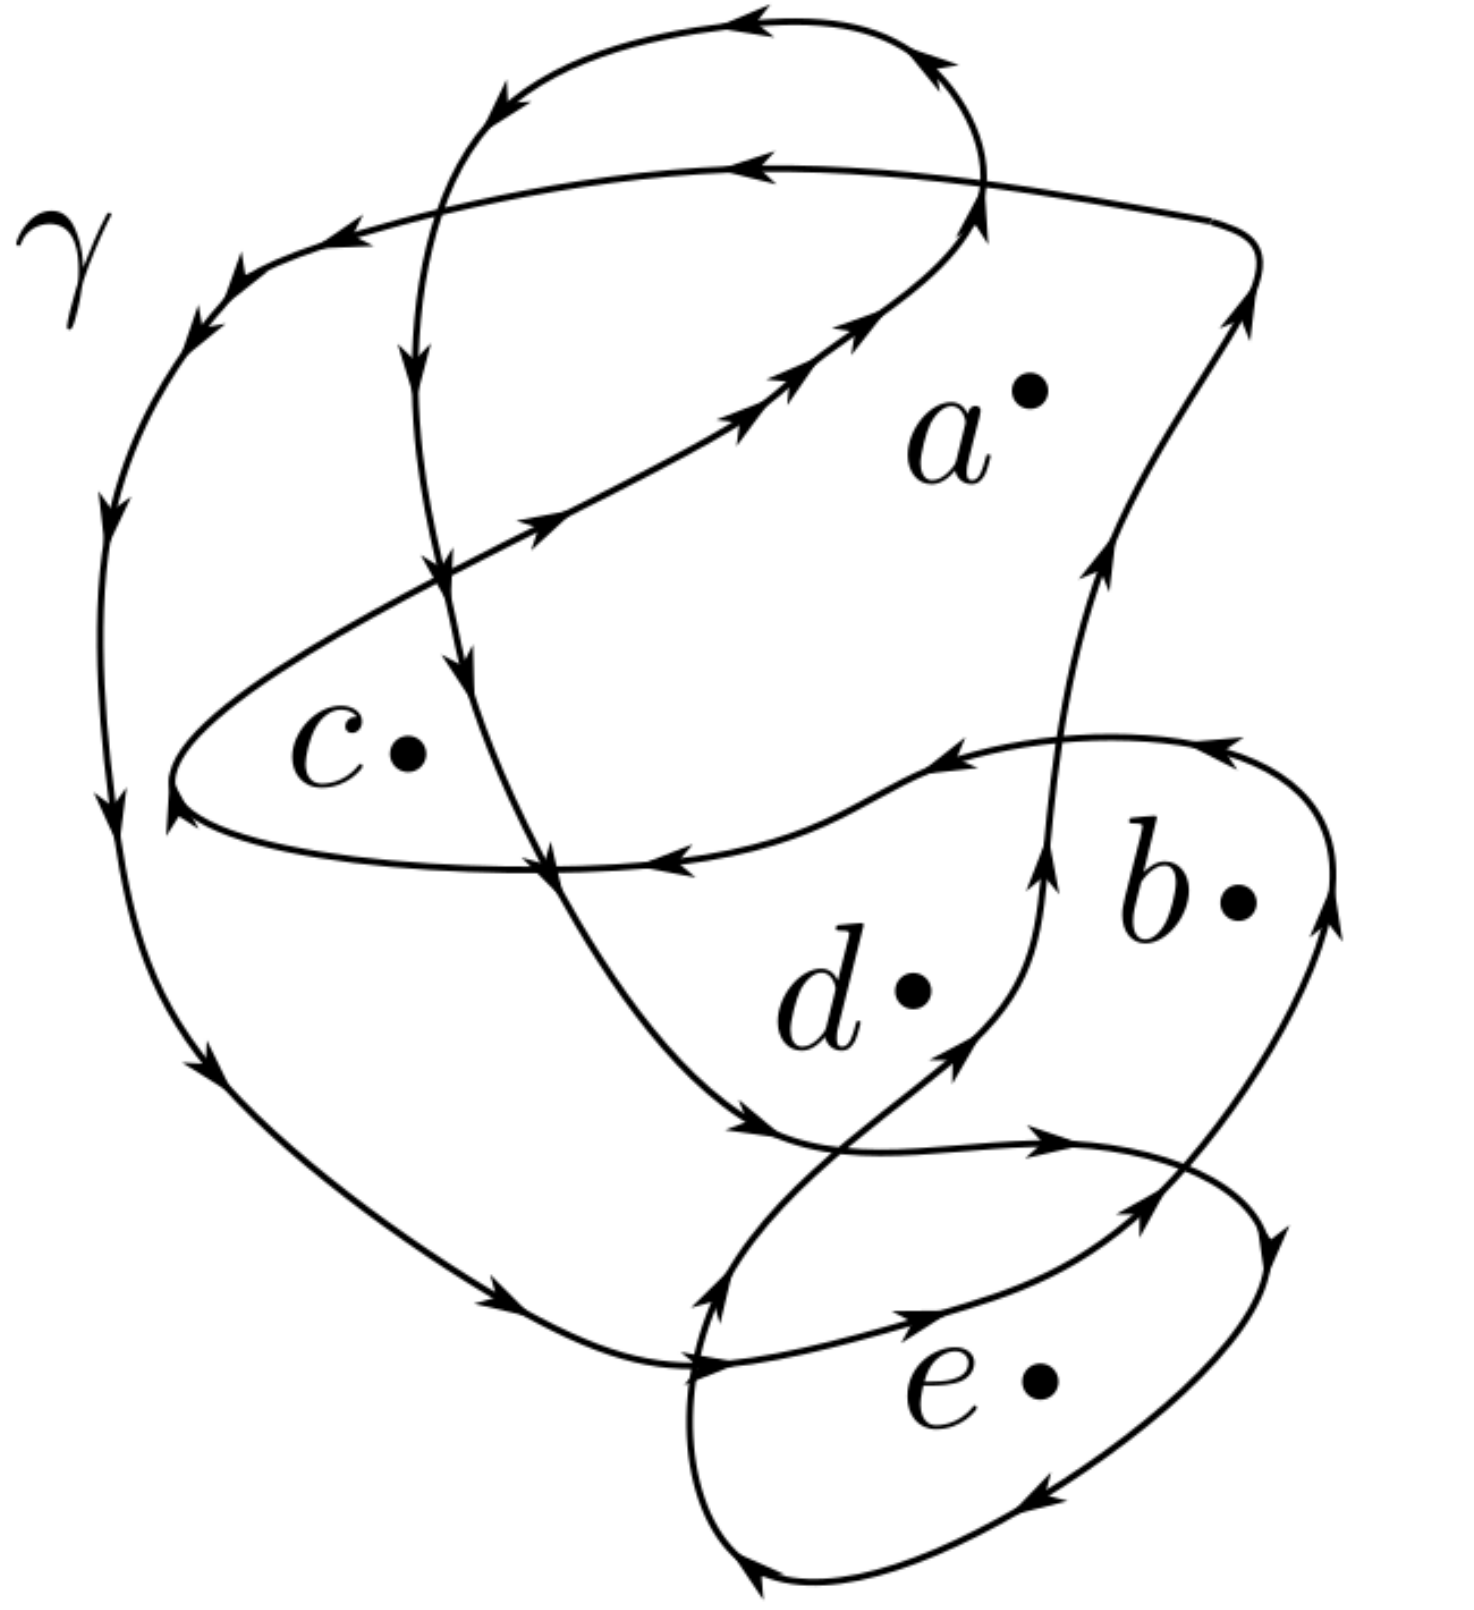
\includegraphics[width=7cm]{sheet 2 q 8}\end{center}



\question%9 yippee cool integrals :3 but i'm not sure why they have the b>0 condition, both sides are even functions of b and the result certainly holds when b=0, so it should hold for all b in R
Let $f(z)=\exp(-z^2)$. Using an appropriate contour and applying the Cauchy-Goursat theorem to $f$, show that \[
	\int_0^\infty e^{-x^2}\cos(2bx)\mathrm{~d}x=\frac{\sqrt\pi}2e^{-b^2},\qquad b>0.
\] You may use that $\int_0^\infty e^{-x^2}\mathrm{~d}x=\sqrt\pi/2$. [\emph{Hint: note that $f(x+iy)=\exp(y^2)\exp(-x^2)(\cos(2xy)-i\sin(2xy))$.}]



\question%10
(Extra challenge) Let $U$ be a simply connected domain and $f$ be a holomorphic function in $U$ which does not vanish anywhere. Show that it is possible to define a branch of $\log f$ in $U$. Give an example showing that it might be impossible to define a branch of $\log$ on $f(U)$.

\end{questions}

\end{document}
